\documentclass[../Main.tex]{subfiles}

\begin{document}
\chapter{Случайные события}

\section{Понятие случайного события}

Предметом исследования в теории вероятностей являются \textbf{события}, появляющиеся при определенных условиях, которые можно воспроизводить неограниченное количество раз. Эти условия называются \textbf{испытание, опыт}.

\defn{Событие}{
Явление, которое происходит в результате осуществления определенного комплекса условий.
}

\defn{Эксперимент (опыт, испытание)}{
Комплекс условий, которые можно воспроизводить неограниченное количество раз.
}

\section{Классификация событий}
\begin{itemize}
    \item Невозможное событие - то, которое не может произойти в рамках испытания.
    \item Достоверное событие - то, которое точно произойдет в рамках испытания.
    \item Случайное событие - то, которое может произойти или не произойти в рамках эксперимента:
    \begin{itemize}
        \item Совместные события - те, которые в рамках эксперимента могут произойти одновременно.
        \item Несовместные события - те, которые не могут произойти одновременно в рамках одного эксперимента (появление одного из них исключает появление второго)
        \item Равновозможные события - те, которые в рамках эксперимента происходят с одинаковой частотой.
        \item Противоположные события - непоявление одного из них в рамках эксперимента влечет появление другого.
    \end{itemize}
\end{itemize}

\defn{Полная группа событий}{
В результате эксперимента обязательно должно произойти хотя бы одно из них и любые два из них несовместны.
}

\defn{Элементарные исходы}{
Такие исходы, которые не могут быть разделены на другие в рамках данного эксперимента.
}

\defn{Благоприятные исходы}{
Элементарные исходы, образующие данное событие.
}

\section{Операции над событиями}
\begin{enumerate}
    \item A=B: (равенство) - если появление A влечет за собой появление B, а B - влечет A (не обязательно совпадают).
    \item \(A+B (A \bigcup B)\): сумма (объединение) - появление хотя бы одного из событий.
    \begin{center}
        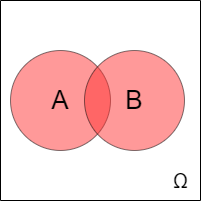
\includegraphics[width=0.25\linewidth]{сумма.png}
    \end{center}
    \item \(A \cdot B (A \bigcap B)\): произведение (пересечение) - осуществление обоих событий.
    \begin{center}
        
\includegraphics[width=0.25\linewidth]{произв.png}
    \end{center}
    \item \(A \setminus B\): разность - происходит A, но не происходит B.
    \begin{center}
        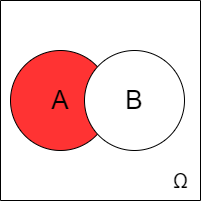
\includegraphics[width=0.25\linewidth]{разность.png}
    \end{center}
\end{enumerate}

\section{Классическая формула вероятности}

\defn{Вероятность}{
Вероятностью события А называется математическая оценка возможности появления этого события в результате опыта, равная отношению числа, благоприятствующих событию А исходов опыта к общему числу равновозможных попарно несовместных исходов опыта, образующих полную группу событий.
}

\[P(A) = \dfrac{M}{N},\]
где N - число всех исходов испытания, а M - число исходов, благоприятствующих событию A.

\subsection*{Общая схема решения задач}
\begin{enumerate}
    \item Определить, в чем состоит случайный эксперимент и какие у него элементарные события (исходы). Убедиться, что они равновозможны;
    \item Найти общее число элементарных событий N;
    \item Определить, какие элементарные события благоприятствуют интересующему нас событию А, и найти их число M;
    \item Найти вероятность события А по формуле \(P(A) = \dfrac{M}{N}\).
\end{enumerate}

\section{Геометрическая вероятность}

\defn{Геометрическое определение вероятности}{
Если предположить, что попадание в любую точку области \(\Omega\) равновозможно, то вероятность попадания случайной точки в заданное множество А будет равна отношению площадей
\[P(A) = \dfrac{S(A)}{S(\Omega)}.\]
}

Если А имеет нулевую площадь, то вероятность попадания в А равна нулю.

Можно определить геометрическую вероятность в пространстве и на прямой:
\[P(A) = \dfrac{V(A)}{V(\Omega)}, P(A) = \dfrac{L(A)}{L(\Omega)}.\]

\end{document}
